\section{Selection of Coarse Grid Nodes and Prolongation Operator Sparsity}
\label{sec:p_sparsity}
In this chapter, I will present a multigrid method for solving linear elasticity problems discretized with 3D eight-node brick elements on a Cartesian grid. Therefore, the position of node $(i,j,k)$ in undeformed space $\mathbf{X}$, can be written as:
$$
\mathbf{X}(i,j,k) = (i*h,j*h,k*h), (i,j,k) \in G^0
$$
Here, $h$ is the element length. $G^0$ is the finest level discretization.We wish to maintain the regularity across all levels. Therefore, we can write the position of node $(i,j,k)$ in undeformed space $\mathbf{X}$ at level 1 as:
$$
\mathbf{X}(i,j,k) = (i*2h,j*2h,k*2h), (i,j,k) \in G^1
$$
And so on for the coarser levels. Now that we have selected the coarse grid degrees of freedom, a proper prolongation operator is required for building the multigrid hierarchy. Given that the finest level operator $\mathbf{L}^0$ has a regular $27$ point stencil sparsity, we wish that all coarse level operators $\mathbf{L}^c$ shares the same sparsity. Here I will propose a sparsity pattern for the prolongation operator that guarantees such property, though it is not the only one that satisfies, but it is most commonly used, and fits well with the methods for computing the prolongation operator in the next sections.
\begin{enumerate}
\item If a fine node $f$ is coincide with a coarse node $c$ in undeformed space, $P_{fc^*} = 0$, if $c^* \neq c$
\item If a fine node $f$ lies on a coarse element edge in undeformed space. If coarse node $c_1$ and $c_2$ define this edge, $P_{fc^*} = 0$, if $c^* \neq c_1$ and $c^* \neq c_2$, Figure~\ref{fig:neighbor_ring}.
\item If a fine node $f$ lies on a coarse element face in undeformed space. If coarse node $c_1$, $c_2$, $c_3$, and $c_4$ define this face, $P_{fc^*} = 0$, if $c^* \neq c_p$, $\forall c_p \in \{c_1,c_2,c_3,c_4\}$.
\item If a fine node $f$ lies on a coarse element center in undeformed space. If coarse node $c_1$, $c_2$, $c_3$, $c_4$, $c_5$, $c_6$, $c_7$, and $c_8$ define this coarse element, $P_{fc^*} = 0$, if $c^* \neq c_p$, $\forall c_p \in \{c_1,c_2,c_3,c_4,c_5,c_6,c_7,c_8\}$.
\end{enumerate}
 Note that these rules create same coarse nodes and prolongation operators that is of exact same sparsity as a standard multilinearly interpolated prolongation operators in Chapter~\ref{Chapter:Elasticity}.
\section{Building Prolongation Operator Using Local Problems}
\subsection{Define Local Matrix}
In section~\ref{sec:Convergence_Metric}, we stated that the quality of the prolongation operator can be measured by two metrics:
 \begin{equation}
M_1(\mathbf{Q},\mathbf{e}) := \frac{<(\mathbf{I}-\mathbf{Q})\mathbf{e}, (\mathbf{I}-\mathbf{Q})\mathbf{e}>}{<\mathbf{L}\mathbf{e},\mathbf{e}>}
\end{equation}
\begin{equation}
M_2(\mathbf{Q},\mathbf{e}) := \frac{<\mathbf{L}(\mathbf{I}-\mathbf{Q})\mathbf{e}, (\mathbf{I}-\mathbf{Q})\mathbf{e}>}{<\mathbf{L}\mathbf{e},\mathbf{e}>}
\end{equation}
Here we take $\mathbf{Q}$ as:
$$
  \mathbf{Q} = \left[ \begin{array}{cc}
    \mathbf{0} & \mathbf{P}_{cf} \\
    \mathbf{0} & \mathbf{I}_c
  \end{array}\right]\\
$$
But both measurement requires the global operator $\mathbf{L}$. In work \cite{brezina2001algebraic}, an alternative local operator $\mathbf{L}_i$ is proposed. $\mathbf{L}_i$ is the sum of the element stiffness matrix adjacent to a given fine node $i$.
\begin{equation}
\mathbf{L}_i = \sum_{\alpha\in \mathcal{T}_i} L_\alpha
\label{equ:local_matrix}
\end{equation}
$L_\alpha$ is the elemental stiffness matrix of element $\alpha$, $\mathcal{T}$ is one ring neighborhood, illustrated in Figure~\ref{fig:neighbor_ring}.
\begin{figure}[t]
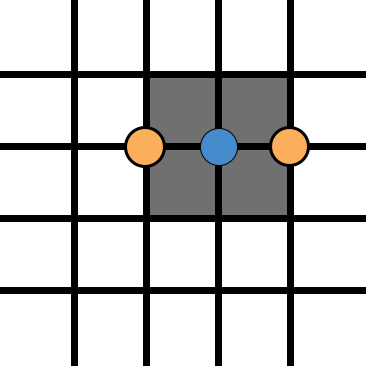
\includegraphics[width=4cm]{BBMG/neighbor.png}
\centering
\caption{A neighborhood of a given fine node, shaded in blue, in Cartesian discretization. The neighboring cells of the given node is shaded in gray. In this case, we are interpolating the fine node values from the given coarse nodes, shaded in yellow.}
\label{fig:neighbor_ring}
\end{figure}
The localized measurement $M_{i,1}$ and $M_{i,2}$ can then be defined as:
 \begin{equation}
M_{i,1}(\mathbf{Q},\mathbf{e}) := \frac{<\epsilon_i\epsilon^T_i(\mathbf{I}-\mathbf{Q})\mathbf{e}, \epsilon_i\epsilon^T_i(\mathbf{I}-\mathbf{Q})\mathbf{e}>}{<\mathbf{L}_i\mathbf{e},\mathbf{e}>}
\end{equation}
\begin{equation}
M_{i,2}(\mathbf{Q},\mathbf{e}) := \frac{<\mathbf{L}_i\epsilon_i\epsilon^T_i(\mathbf{I}-\mathbf{Q})\mathbf{e}, \epsilon_i\epsilon^T_i(\mathbf{I}-\mathbf{Q})\mathbf{e}>}{<\mathbf{L}_i\mathbf{e},\mathbf{e}>}
\end{equation}
Here $\epsilon_i$ is a vector, that its entries satisfies:
$$
\epsilon_i(j) = \delta_{ij} 
$$
$\delta$ is the Kronecker delta. If we denote the set of projection operators $\mathbf{Q}$ that satisfies those sparsity conditions stated in section~\ref{sec:p_sparsity} as $\mathcal{Z}_i$. The $i$th row if $\mathbf{Q}$ is then:
$$
\mathbf{q}^T_i = \epsilon^T_i\mathbf{Q}
$$
 Then finding the prolongation operator for a given fine node $i$ can be expressed as the following min-max problem:
 \begin{align}
 K_{i,p} = \min_{q_i \in \mathcal{Z}_i} \max_{\mathbf{e}\perp \text{Null}(\mathbf{L}_i)} M_{i,p}(\mathbf{q}_i,\mathbf{e})\nonumber\\
 \text{subject to } (\epsilon_i - \mathbf{q}_i) ^ T \mathbf{e} = 0\text{, }\forall \mathbf{e} \in \text{Null}(\mathbf{L}_i) \label{equ:local_metric}
 \end{align}
 The condition in equation~\ref{equ:local_metric}, states that the prolongation operator must correctly interpolate local null space. For Poisson problems, the nullity of the local matrix is only 1. But for elasticity problems the nullity of the local matrix is drastically raised to 6 in 3D. Three degrees of displacements and three degrees rotations. 
 \subsection{Computation of the Prolongation Operator}
 For the local problem defined above with fine node $i$, we denote the set of nodes included in this local problem as $\mathcal{N}_i$. We write $c$ as the coarse nodes that fine node $i$ is interpolated from. $f$ as the fine nodes from $\mathcal{N}_i$. $n_c$ is the size of the set $c$, and $n_f$ is the size of the set $f$. Then we can write the local matrix $L_i$ as:
 $$
\mathbf{L}_i = \begin{bmatrix} 
 \mathbf{L}^{(1)}_{ff} & \mathbf{L}^{(1)}_{fc} \\
 \mathbf{L}^{(1)}_{cf} & \mathbf{L}^{(1)}_{cc}
 \end{bmatrix}
 $$
 for metric $M_{i,1}$, and:
  $$
 \mathbf{L}^2_i = \begin{bmatrix} 
 \mathbf{L}^{(2)}_{ff} & \mathbf{L}^{(2)}_{fc} \\
 \mathbf{L}^{(2)}_{cf} & \mathbf{L}^{(2)}_{cc}
 \end{bmatrix}
 $$
 for metric $M_{i,2}$. If we place node $i$ as the first of all the nodes $f$. we can replace $\epsilon_i$ with $\epsilon_1$ in the two local metrics. 
 
\begin{lem}\label{lemma:q_existance}There exits $\mathbf{q}_i \in \mathcal{Z}_i$, such that $\epsilon_1 - \mathbf{q}_i \in \text{Range}(\mathbf{L}^p_i)$ if and only if
$$
\hat{\epsilon}_1 \in \text{Range}(\mathbf{L}^{(p)}_{ff})
$$
$\hat{\epsilon}_1$ is the first canonical basis vector of length $n_f$. $p = 1\text{ or }2$.
\end{lem}
Lemma~\ref{lemma:q_existance} simply state that there exists an interpolation that interpolates null space correctly, if the fine node $i$ does not have a zero diagonal.
\begin{theorem}
\label{theo:p_solution}
If $\hat{\epsilon}_1 \in \text{Range}(\mathbf{L}^{(p)}_{ff})$, than $K_{i,p} = \infty$. If $\hat{\epsilon}_1 = \mathbf{L}^{(p)}_{ff} \hat{\delta}_1$, then the unique solution of equation~\ref{equ:local_metric} is given by
\begin{equation}
\mathbf{q}_i^* = \left(\begin{array}{c}0 \\ -\mathbf{L}^{(p)}_{cf}\hat{\delta}_1\end{array}\right)  \in \mathcal{Z}
\end{equation}
and $K_{i,p} = <\hat{\epsilon}_1,\hat{\delta}_1>$, for $p = 1\text{ or }2$.
\end{theorem} 
First part of Theorem~\ref{theo:p_solution} states that if there is no solution exists, multigrid can not converge for the error mode containing node $i$. From Lemma~\ref{lemma:q_existance}, there is no solution if node $i$ has zero diagonal. Therefore any error modes that has a non-zero error for node $i$, is in the null space of the original matrix, then there is no solution to the original matrix.

Second part of Theorem~\ref{theo:p_solution}, states how we can compute the prolongation operator:
\begin{align}
\hat{\epsilon}_1 &= \mathbf{L}^{(p)}_{ff}\hat{\delta}_1 \nonumber \\
\hat{\delta}_1 &= (\mathbf{L}^{(p)}_{ff})^{(-1)}\hat{\epsilon}_1 \nonumber \\
\mathbf{q}_i^* &= (\mathbf{e}^T_i\mathbf{Q})^T \nonumber \\
&= \mathbf{Q}^T\epsilon_i \nonumber \\
&= \left(\begin{array}{c} 0 \\ \mathbf{P}^T_{fc}\epsilon_i\end{array}\right) \nonumber \\
&= \left(\begin{array}{c}0 \\ -\mathbf{L}^{(p)}_{cf}\hat{\delta}_1\end{array}\right) \nonumber \\
\mathbf{P}^T_{fc}\epsilon_i &=  -\mathbf{L}^{(p)}_{cf}\hat{\delta}_1 \nonumber \\
&= -\mathbf{L}^{(p)}_{cf}(\mathbf{L}^{(p)}_{ff})^{-1}\hat{\epsilon}_1 \label{equ:p_solution}
\end{align}
$\mathbf{P}^T_{fc}\epsilon_i$ is a row of the prolongation operator. A practical way for computing it when using metric $M_{i,1}$, is to set the coarse nodes in the local problem as Dirichlet. By setting each degrees of freedom $j$ with value of $1$, i.e. a Kronecker delta. Solving the local problem, the value(s) of the DOF of fine node $i$ is then the entry $\epsilon^T_i\mathbf{P}_{fc}\epsilon_j$.
Here each row of the prolongation operator is the harmonic extension of a canonical basis vector.
If reader are interested in the proof of Lemma~\ref{lemma:q_existance} and Theorem~\ref{theo:p_solution}, I refer reader to \cite{brezina2001algebraic}. Here, I will only use the result and viewing their implications. Furthermore, it is worth noting that in work \cite{henson2001element}, an alternative formulation of equation~\ref{equ:local_metric} in the perspective of energy minimization was proposed, upon which work \cite{dohrmann2007interpolation} was based. As it is unimportant for the derivation of our method, I will omit that formulation here.